\subsection{Overview}
%%%%%%%%%%%%%%%%%%%%%%%%%%%%%%%%%%%%%%%%%%%%%%%%%%%%%%%%%%
\frame {\frametitle{Amazon Web Services}
%%%%%%%%%%%%%%%%%%%%%%%%%%%%%%%%%%%%%%%%%%%%%%%%%%%%%%%%%%
\begin{itemize}
	\item {\bf Amazon's cloud computing services}
	\begin{itemize}
		\item S3, EC2, RedShift, SimpleDB, Elastic MR, and many, many more
		\item Combined, they allow constructing Internet-scale applications
	\end{itemize}

	\vspace{40pt}

	\item {\bf Infrastructure services requirements:}
	\begin{itemize}
		\item Security, scalability, availability, performance, cost-efficiency
		\item Serve millions of customers worldwide, continuously
	\end{itemize}
\end{itemize}
}

%%%%%%%%%%%%%%%%%%%%%%%%%%%%%%%%%%%%%%%%%%%%%%%%%%%%%%%%%%
\frame {\frametitle{Amazon Web Services}
%%%%%%%%%%%%%%%%%%%%%%%%%%%%%%%%%%%%%%%%%%%%%%%%%%%%%%%%%%
\begin{itemize}
	\item {\bf Important observations}
	\begin{itemize}
		\item No emphasis on consistency
		\item AWS is in AP, sacrificing consistency
	\end{itemize}

	\vspace{40pt}

	\item {\bf AWS follows the BASE philosophy}
	\begin{itemize}
		\item BASE vs. ACID
		\item Basically Available
		\item Soft state
		\item Eventually consistent
	\end{itemize}
\end{itemize}
}

%%%%%%%%%%%%%%%%%%%%%%%%%%%%%%%%%%%%%%%%%%%%%%%%%%%%%%%%%%
\frame {\frametitle{Why favoring Availability over Consistency?}
%%%%%%%%%%%%%%%%%%%%%%%%%%%%%%%%%%%%%%%%%%%%%%%%%%%%%%%%%%
\begin{itemize}
	\item {\bf Even the shortest outage has significant financial consequences and impact customer trust}

	\vspace{40pt}

	\item {\bf Clearly, consistency violations may as well have a big impact}
	\begin{itemize}
		\item But not in several Amazon's services
		\item {\color{red} Billing} is a separate story
	\end{itemize}
\end{itemize}
}

%%%%%%%%%%%%%%%%%%%%%%%%%%%%%%%%%%%%%%%%%%%%%%%%%%%%%%%%%%
\frame {\frametitle{Amazon Dynamo}
%%%%%%%%%%%%%%%%%%%%%%%%%%%%%%%%%%%%%%%%%%%%%%%%%%%%%%%%%%
\begin{itemize}
	\item {\bf Works behind the scenes in the context of AWS}
	\begin{itemize}
		\item Used to power client-facing services such as S3, and others
		\item Used to power internal Amazon services such as: shopping cart, customer session management, product catalog, recommendations, order fulfillment, sales rank, fraud detection, ...
	\end{itemize}

	\vspace{40pt}

	\item {\bf What is Dynamo?}
	\begin{itemize}
		\item Highly available key-value storage system
		\item Favors availability over consistency under failures
	\end{itemize}
\end{itemize}
}

%%%%%%%%%%%%%%%%%%%%%%%%%%%%%%%%%%%%%%%%%%%%%%%%%%%%%%%%%%
\frame {\frametitle{What is a key-value store?}
%%%%%%%%%%%%%%%%%%%%%%%%%%%%%%%%%%%%%%%%%%%%%%%%%%%%%%%%%%
\begin{itemize}
	\item {\bf Think about Hash tables or dictionaries}
	\begin{itemize}
		\item Simple API: \texttt{\bf get(key)}, \texttt{\bf put(key, value)}
		\item Sometimes referred to read/write operations
	\end{itemize}

	\vspace{20pt}

	\item {\bf Specifics of Dynamo API}
	\begin{itemize}
		\item Uses an additional argument to pass a ``context''
		\item Context holds critical metadata
		\item Typically stores {\color{red}small objects} (< 1 MB)
	\end{itemize}

	\vspace{20pt}

	\item {\bf Specifics of services using Dynamo}
	\begin{itemize}
		\item Do not need transactions
		\item Often need only primary-key access to data
	\end{itemize}
\end{itemize}
}

%%%%%%%%%%%%%%%%%%%%%%%%%%%%%%%%%%%%%%%%%%%%%%%%%%%%%%%%%%
\frame {\frametitle{Amazon Dynamo: Features}
%%%%%%%%%%%%%%%%%%%%%%%%%%%%%%%%%%%%%%%%%%%%%%%%%%%%%%%%%%
\begin{itemize}
	\item {\bf Main characteristics}
	\begin{itemize}
		\item Low latency
		\item Scalable (hundreds of machines)
		\item Always-on available (especially for writes)
		\item Partition/Fault tolerance
		\item {\color{red}Eventually} consistent
	\end{itemize}

	\vspace{40pt}

	\item {\bf How such features are obtained}
	\begin{itemize}
		\item General distributed systems toolbox
		\item We review some of them here
	\end{itemize}
\end{itemize}
}

%%%%%%%%%%%%%%%%%%%%%%%%%%%%%%%%%%%%%%%%%%%%%%%%%%%%%%%%%%
\frame {\frametitle{Amazon Dynamo: Key Techniques (1)}
%%%%%%%%%%%%%%%%%%%%%%%%%%%%%%%%%%%%%%%%%%%%%%%%%%%%%%%%%%
\begin{itemize}
	\item {\bf Consistent hashing} [Karger97]
	\begin{itemize}
		\item For data partitioning, replication and load balancing
	\end{itemize}

	\vspace{40pt}

	\item {\bf Sloppy Quorums}
	\begin{itemize}
		\item Boosts availability in presence of failures
		\item May result in inconsistent versions of keys (data)
	\end{itemize}
\end{itemize}
}

%%%%%%%%%%%%%%%%%%%%%%%%%%%%%%%%%%%%%%%%%%%%%%%%%%%%%%%%%%
\frame {\frametitle{Amazon Dynamo: Key Techniques (2)}
%%%%%%%%%%%%%%%%%%%%%%%%%%%%%%%%%%%%%%%%%%%%%%%%%%%%%%%%%%
\begin{itemize}
	\item {\bf Vector clocks} [Fidge88/Mantern88]
	\begin{itemize}
		\item For tracking causal dependencies among different versions of the same key (data)
	\end{itemize}

	\vspace{20pt}

	\item {\bf Gossip-based group membership}
	\begin{itemize}
		\item For maintaining information about alive nodes
	\end{itemize}

	\vspace{20pt}

	\item {\bf Anti-entropy protocol based on Merkle trees}
	\begin{itemize}
		\item Background synchronization of divergent replicas
	\end{itemize}
\end{itemize}
}

%%%%%%%%%%%%%%%%%%%%%%%%%%%%%%%%%%%%%%%%%%%%%%%%%%%%%%%%%%
\frame {\frametitle{Amazon Dynamo: Design Decisions}
%%%%%%%%%%%%%%%%%%%%%%%%%%%%%%%%%%%%%%%%%%%%%%%%%%%%%%%%%%
\begin{itemize}
	\item {\bf Always writable data store}
	\begin{itemize}
		\item E.g., think shopping cart service
	\end{itemize}

	\vspace{20pt}

	\item {\bf How to handle data changes?}
	\begin{itemize}
		\item Replication, required for fault/disaster tolerance
		\item Allow multiple versions of data
		\item Reconcile and resolve conflicts {\color{red}during reads}
	\end{itemize}

	\vspace{20pt}

	\item {\bf How to reconcile data?}
	\begin{itemize}
		\item Application-side: depending on business logic
		\item Dynamo: deterministic, e.g., ``last-write'' wins
	\end{itemize}
\end{itemize}
}




\subsection{Dynamo Architecture}
%%%%%%%%%%%%%%%%%%%%%%%%%%%%%%%%%%%%%%%%%%%%%%%%%%%%%%%%%%
%%%%%%%%%%%%%%%%%%%%%%%%%%%%%%%%%%%%%%%%%%%%%%%%%%%%%%%%%%
\begin{frame}
 \begin{colorblock}{blue}{lightblue}{ }
  \begin{center}
    \textbf{\texttt{Amazon Dynamo: Architecture}}
  \end{center}
  \end{colorblock}
\end{frame}
%%%%%%%%%%%%%%%%%%%%%%%%%%%%%%%%%%%%%%%%%%%%%%%%%%%%%%%%%%
%%%%%%%%%%%%%%%%%%%%%%%%%%%%%%%%%%%%%%%%%%%%%%%%%%%%%%%%%%

%%%%%%%%%%%%%%%%%%%%%%%%%%%%%%%%%%%%%%%%%%%%%%%%%%%%%%%%%%
\frame {\frametitle{Amazon Dynamo Architecture}
%%%%%%%%%%%%%%%%%%%%%%%%%%%%%%%%%%%%%%%%%%%%%%%%%%%%%%%%%%
\begin{itemize}
	\item {\bf Scalable and robust components for:}
	\begin{itemize}
		\item {\bf Load balancing and data partitioning}
		\item {\bf Membership, fault detection}
		\item Failure recovery
		\item {\bf Replica synchronization}
		\item Overload Handling
		\item State transfer
		\item Concurrency management
		\item Scheduling
		\item Request marshalling and routing
		\item System monitoring
		\item Configuration management
	\end{itemize}

\end{itemize}
}

\subsection{Data Partitioning}
%%%%%%%%%%%%%%%%%%%%%%%%%%%%%%%%%%%%%%%%%%%%%%%%%%%%%%%%%%
\frame {\frametitle{Amazon Dynamo: Data Partitioning}
%%%%%%%%%%%%%%%%%%%%%%%%%%%%%%%%%%%%%%%%%%%%%%%%%%%%%%%%%%
\begin{itemize}
	\item {\bf Data partitioning}
	\begin{itemize}
		\item Dynamic partitioning of {\color{red}keys} over a set of storage {\color{red}nodes}
		\item Technique used for DHTs, e.g., Chord
	\end{itemize}

	\vspace{20pt}

	\item {\bf Consistent Hashing}
	\begin{itemize}
		\item Hashes of keys give key $m$-bit identifiers
		\item Hashes of nodes give $m$-bit identifiers
		\item Identifiers are ordered in an identifier circle
	\end{itemize}

	\vspace{20pt}

	\item {\bf Key assignment to storage nodes}
	\begin{itemize}
		\item A key is assigned to the closest {\color{red}successor node} ID
		\item Key $k$ is assigned to the first node whose ID $\geq k$
		\item If such node does not exist, navigate the circle and find node with the smallest ID
	\end{itemize}
\end{itemize}
}

%%%%%%%%%%%%%%%%%%%%%%%%%%%%%%%%%%%%%%%%%%%%%%%%%%%%%%%%%%
\frame {\frametitle{Consistent Hashing Example}
%%%%%%%%%%%%%%%%%%%%%%%%%%%%%%%%%%%%%%%%%%%%%%%%%%%%%%%%%%
\begin{itemize}
	\item Assume: $m=3$ bit, 3 storage nodes (0,2,3), 4 keys (1,3,5,6)
\end{itemize}
\begin{figure}[h]
	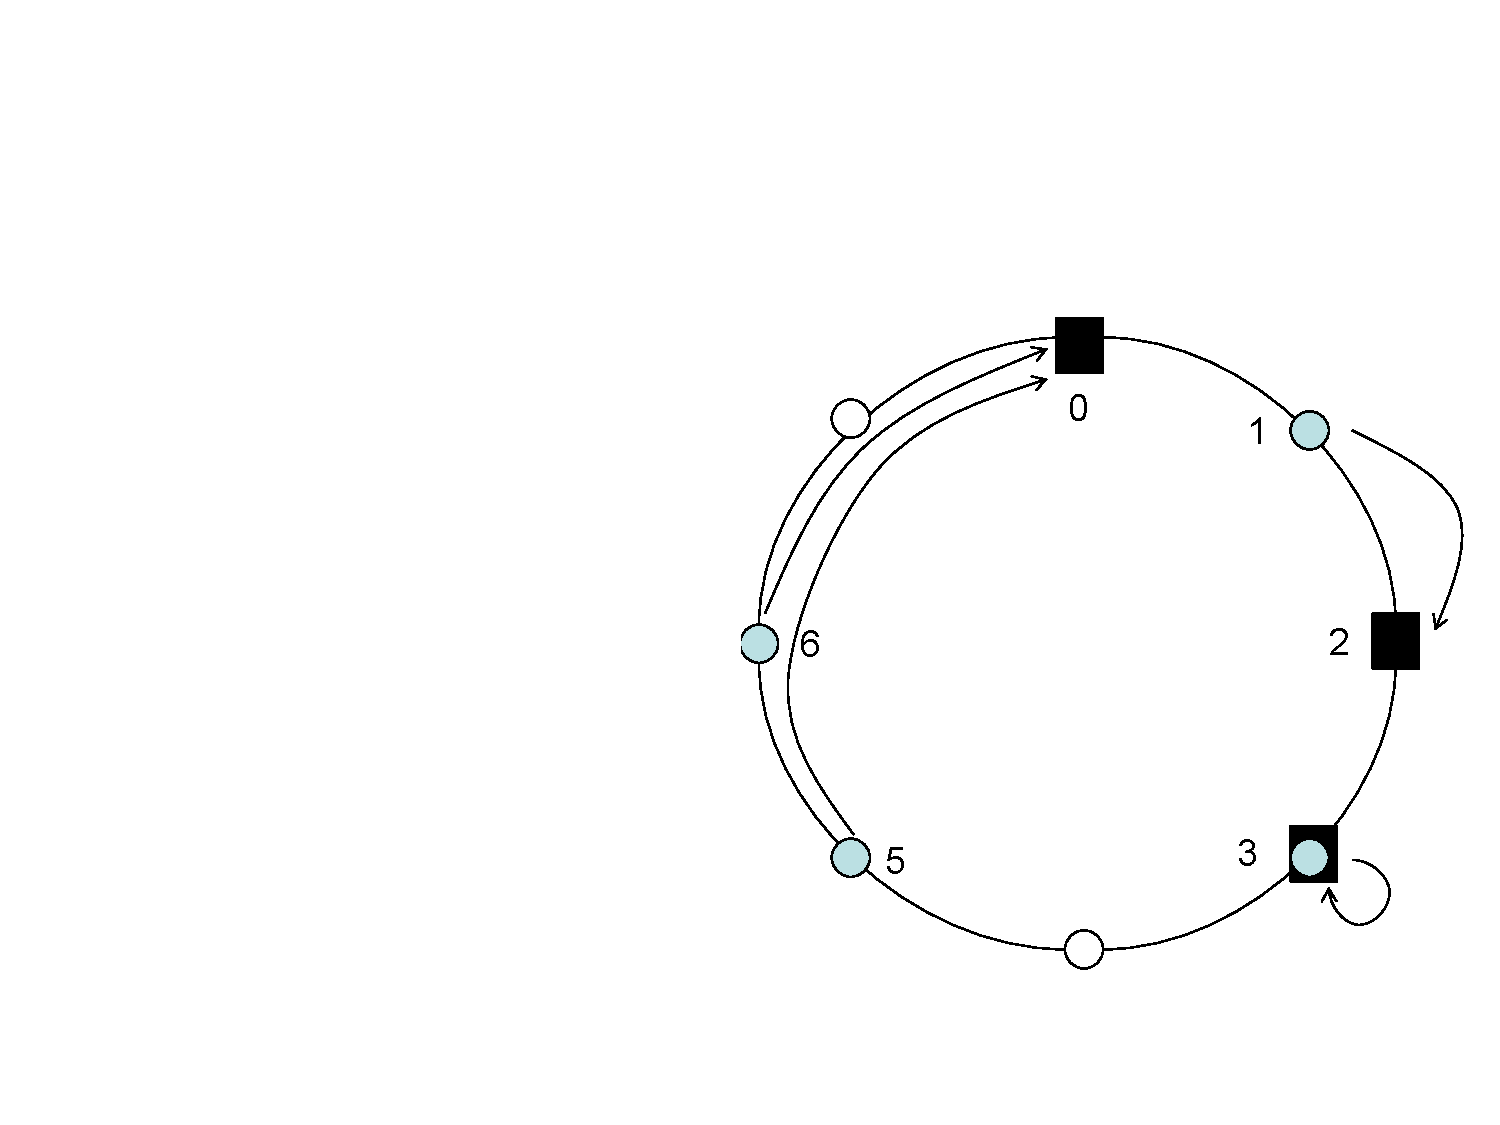
\includegraphics[scale=0.3]{./figures/consistent_hashing_example}
\end{figure}
}

%%%%%%%%%%%%%%%%%%%%%%%%%%%%%%%%%%%%%%%%%%%%%%%%%%%%%%%%%%
\frame {\frametitle{Consistent Hashing: Key Properties (1)}
%%%%%%%%%%%%%%%%%%%%%%%%%%%%%%%%%%%%%%%%%%%%%%%%%%%%%%%%%%
\begin{itemize}
	\item {\bf Dynamic membership management}
	\begin{itemize}
		\item Storage nodes can come and go
		\item Allows incremental scalability
	\end{itemize}

	\vspace{40pt}

	\item {\bf Storage node arrival/departures}
	\begin{itemize}
		\item \texttt{$n$ Joins}: some (maybe many) keys previously assigned to node $n$'s successor are now assigned to $n$
		\item \texttt{$n$ Leaves}: all keys currently assigned to node $n$ are assigned to its successor
	\end{itemize}
\end{itemize}
}

%%%%%%%%%%%%%%%%%%%%%%%%%%%%%%%%%%%%%%%%%%%%%%%%%%%%%%%%%%
\frame {\frametitle{Consistent Hashing: Key Properties (2)}
%%%%%%%%%%%%%%%%%%%%%%%%%%%%%%%%%%%%%%%%%%%%%%%%%%%%%%%%%%
\begin{itemize}
	\item {\bf Load balancing} [Karger97]
	\begin{itemize}
		\item Each node is responsible for at most $(1+ \epsilon)K/N$ keys
		\item When a new node joins, only $O(K/n)$ keys must be moved (optimal)
	\end{itemize}

	\vspace{40pt}

	\item {\bf Virtual Nodes}
	\begin{itemize}
		\item Each physical storage node mapped multiple times to the circle
		\item[$\to$] Improves load balancing
		\item[$\to$] Allows heterogeneous storage nodes
	\end{itemize}
\end{itemize}
}

\subsection{Data Replication}
%%%%%%%%%%%%%%%%%%%%%%%%%%%%%%%%%%%%%%%%%%%%%%%%%%%%%%%%%%
\frame {\frametitle{Amazon Dynamo: Data Replication}
%%%%%%%%%%%%%%%%%%%%%%%%%%%%%%%%%%%%%%%%%%%%%%%%%%%%%%%%%%
\begin{itemize}
	\item {\bf Goal: achieve high availability and durability}
	\begin{itemize}
		\item Each data item (key) replicated at $N$ nodes
		\item Virtual nodes: same physical node skipped
		\item $N$ is a configurable parameter per Dynamo instance
	\end{itemize}

	\vspace{40pt}

	\item {\bf Example:}
	\begin{itemize}
		\item Assume $N=3$
		\item For key $k$, $B$ is the ``coordinator'' node
		\item $B$ replicates $k$ to $N-1$ other successor nodes (C and D)
		\item[$\to$] $B, C, D$ are a {\bf preference list} for $k$
	\end{itemize}
\end{itemize}
}

\subsection{Data Versioning}
%%%%%%%%%%%%%%%%%%%%%%%%%%%%%%%%%%%%%%%%%%%%%%%%%%%%%%%%%%
\frame {\frametitle{Amazon Dynamo: Data Versioning (1)}
%%%%%%%%%%%%%%%%%%%%%%%%%%%%%%%%%%%%%%%%%%%%%%%%%%%%%%%%%%
\begin{itemize}
	\item {\bf Data replication performed after an ACK is sent to a client \texttt{put} request}
	\begin{itemize}
		\item {\color{red}Asynchronous replication}
		\item May result in inconsistencies under partitions
		\item[$\to$] Read does not return the last value
	\end{itemize}

	\vspace{40pt}

	\item {\bf Operations should not be lost!}
	\begin{itemize}
		\item ``Add to cart'' should not be rejected but also not forgotten
		\item If it is performed when the latest version is not available, then it is performed on a stale version of the data
		\item[$\to$] We may have different version of a key/value pair
	\end{itemize}
\end{itemize}
}

%%%%%%%%%%%%%%%%%%%%%%%%%%%%%%%%%%%%%%%%%%%%%%%%%%%%%%%%%%
\frame {\frametitle{Amazon Dynamo: Data Versioning (2)}
%%%%%%%%%%%%%%%%%%%%%%%%%%%%%%%%%%%%%%%%%%%%%%%%%%%%%%%%%%
\begin{itemize}
	\item {\bf Precautions}
	\begin{itemize}
		\item Once a partition heals, versions are merged
		\item New versions subsume previous ones
		\item Applications {\color{red}must be designed} with data versionin in mind
	\end{itemize}

	\vspace{40pt}

	\item {\bf Key technique for versioning}
	\begin{itemize}
		\item Vector clocks
		\item Capture causality between different versions of an object
	\end{itemize}
\end{itemize}
}

%%%%%%%%%%%%%%%%%%%%%%%%%%%%%%%%%%%%%%%%%%%%%%%%%%%%%%%%%%
\frame {\frametitle{Vector Clocks (in Dynamo) (1)}
%%%%%%%%%%%%%%%%%%%%%%%%%%%%%%%%%%%%%%%%%%%%%%%%%%%%%%%%%%
\begin{itemize}
	\item {\bf In theory:}
	\begin{itemize}
		\item Each \texttt{write} to a key $k$ associated to a vector clock $VC(k)$
		\item $VC(k)$ is an array (map) of integers
		\item In theory, one entry $VC(k)[i]$ for each storage node $i$
		\item When node $i$ handles a write for key $k$ it increments $VC(k)[i]$
	\end{itemize}

	\vspace{40pt}

	\item {\bf In practice:}
	\begin{itemize}
		\item $VC(k)$ will not have many entries $\to$ only node from the preference list should have entries
		\item Dynamo truncates entries if more than a threshold
	\end{itemize}
\end{itemize}
}

%%%%%%%%%%%%%%%%%%%%%%%%%%%%%%%%%%%%%%%%%%%%%%%%%%%%%%%%%%
\frame {\frametitle{Vector Clocks (in Dynamo) (2)}
%%%%%%%%%%%%%%%%%%%%%%%%%%%%%%%%%%%%%%%%%%%%%%%%%%%%%%%%%%
\begin{figure}[h]
	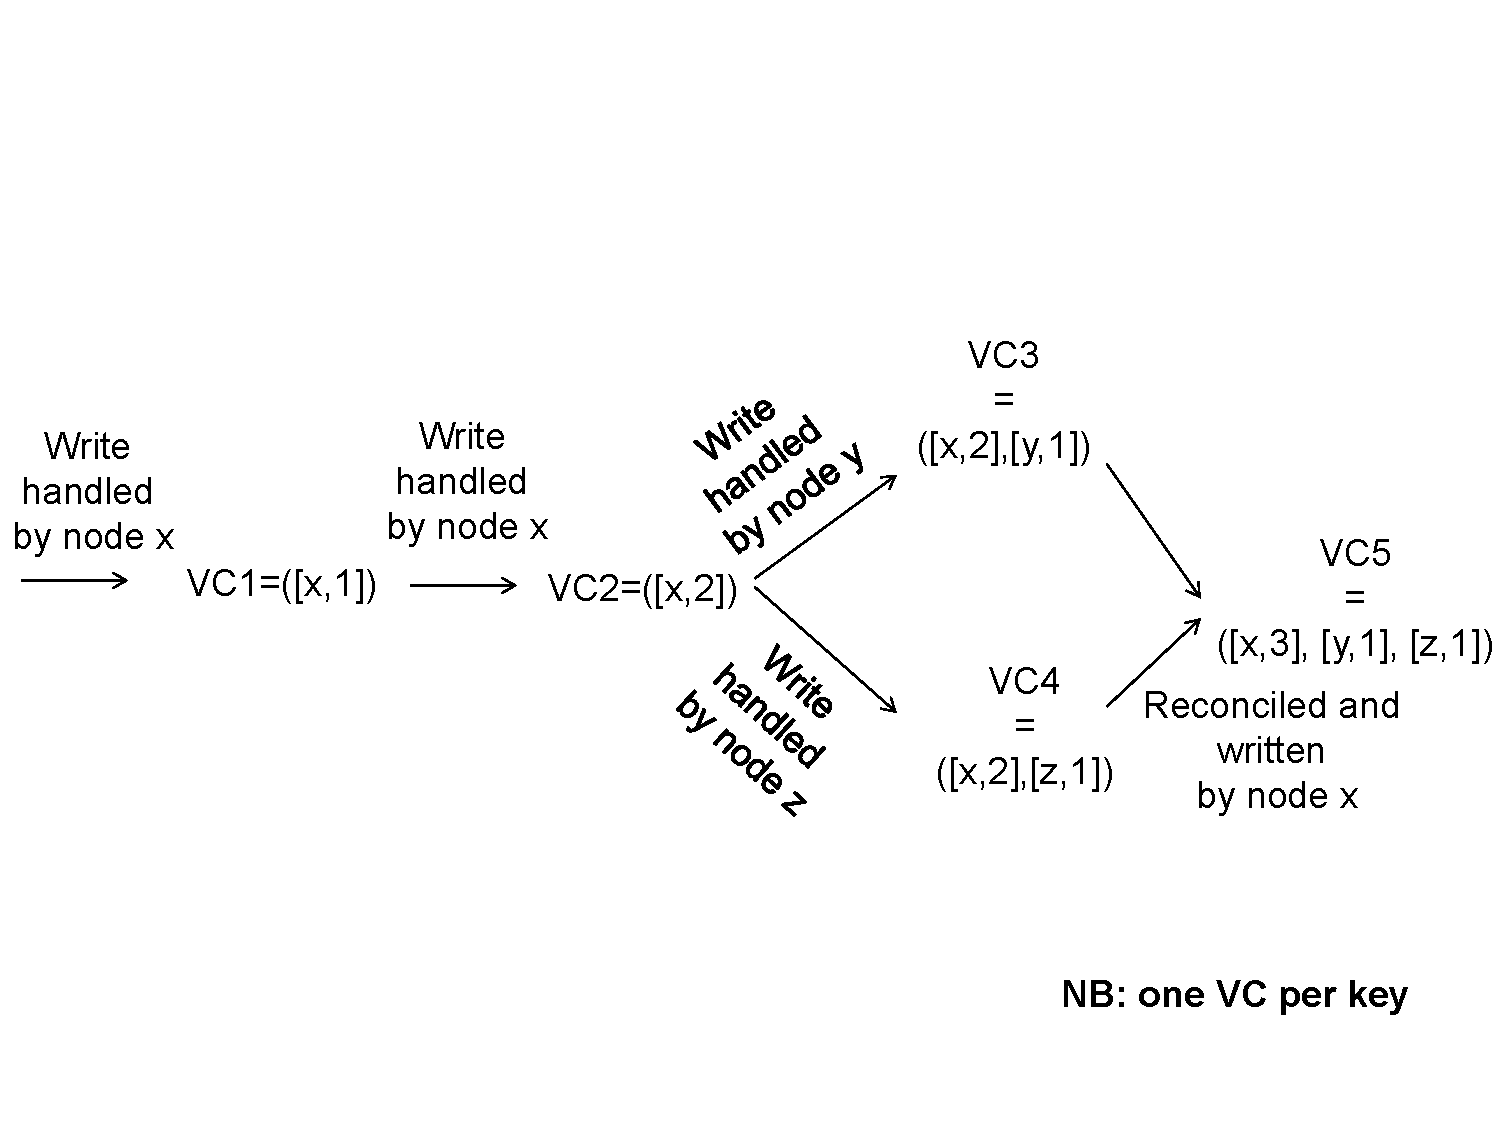
\includegraphics[scale=0.45]{./figures/dynamo_vc_example}
\end{figure}

}

\subsection{Anatomy of put/get}
%%%%%%%%%%%%%%%%%%%%%%%%%%%%%%%%%%%%%%%%%%%%%%%%%%%%%%%%%%
\frame {\frametitle{Anatomy of \texttt{put} and \texttt{get} operations}
%%%%%%%%%%%%%%%%%%%%%%%%%%%%%%%%%%%%%%%%%%%%%%%%%%%%%%%%%%
\begin{itemize}
	\item {\bf Storage nodes can receive requests for {\color{red}any} key}
	\begin{itemize}
		\item Generic load balancer may chose a random node, not necessarily the coordinator
		\item Application may directly contact the coordinator in a preference list
	\end{itemize}

	\vspace{20pt}

	\item {\bf Request routing}
	\begin{itemize}
		\item If request comes from load balancer
		\begin{itemize}
			\item Node serves request only if in preference list
			\item Otherwise, routes the request to the first node in preference list
		\end{itemize}
		\item 0-hop DHT routing: all nodes know all other nodes
		\item[$\to$] Not the most scalable, but excellent for low-latency
	\end{itemize}

	\vspace{20pt}

	\item {\bf Extended preference list}
	\begin{itemize}
		\item Accounts for node failures
	\end{itemize}
\end{itemize}
}

\subsection{Quorums}
%%%%%%%%%%%%%%%%%%%%%%%%%%%%%%%%%%%%%%%%%%%%%%%%%%%%%%%%%%
\frame {\frametitle{Amazon Dynamo: Quorums}
%%%%%%%%%%%%%%%%%%%%%%%%%%%%%%%%%%%%%%%%%%%%%%%%%%%%%%%%%%
\begin{itemize}
	\item {\bf Two important parameters}
	\begin{itemize}
		\item R: number of nodes involved in a get
		\item W: number of nodes involved in a put
		\item Quorum system: $R+W > N$, where $N$ is the number of replicas
	\end{itemize}

	\vspace{20pt}

	\item {\bf Handling put (by coordinator)}
	\begin{itemize}
		\item Generate new VC, write new version locally
		\item Send value, VC, to $N$ nodes from preference list
		\item Wait for $W-1$ acknowledgments
	\end{itemize}

	\vspace{20pt}

	\item {\bf Handling get (by coordinator)}
	\begin{itemize}
		\item Send get to $N$ selected nodes from preference list
		\item Wait for $R$ responses
		\item Select highest versions using VC, reconcile/merge different versions
		\item Writeback reconciled version
	\end{itemize}
\end{itemize}
}

%%%%%%%%%%%%%%%%%%%%%%%%%%%%%%%%%%%%%%%%%%%%%%%%%%%%%%%%%%
\frame {\frametitle{Choosing $R, W$}
%%%%%%%%%%%%%%%%%%%%%%%%%%%%%%%%%%%%%%%%%%%%%%%%%%%%%%%%%%
\begin{itemize}
	\item {\bf $R,W$ smaller than $N$}
	\begin{itemize}
		\item To decrease latency
		\item Slowest replica dictates query latency
	\end{itemize}

	\vspace{20pt}

	\item {\bf $W=1$}
	\begin{itemize}
		\item Always available for writes
		\item Yields $R=N$ $\to$ reads pay the penalty
	\end{itemize}

	\vspace{20pt}

	\item {\bf Typical values in Dynamo}
	\begin{itemize}
		\item $W,R,N = 2,2,3$
	\end{itemize}
\end{itemize}
}

%%%%%%%%%%%%%%%%%%%%%%%%%%%%%%%%%%%%%%%%%%%%%%%%%%%%%%%%%%
\frame {\frametitle{Handling Failures}
%%%%%%%%%%%%%%%%%%%%%%%%%%%%%%%%%%%%%%%%%%%%%%%%%%%%%%%%%%
\begin{itemize}
	\item {\bf $N$ selected nodes are the first $N$ healthy nodes}
	\begin{itemize}
		\item Might change from request to request
		\item Hence the term ``sloppy'' quorums
	\end{itemize}

	\vspace{20pt}

	\item {\bf Sloppy vs. strict quorums}
	\begin{itemize}
		\item Allow availability under a much wider range of partitions
		\item Sacrifice consistency
	\end{itemize}

	\vspace{20pt}

	\item {\bf Data-center wide failures}
	\begin{itemize}
		\item Power outages, cooling failures, network failures, ...
		\item Preference lists account for this
	\end{itemize}
\end{itemize}
}

%%%%%%%%%%%%%%%%%%%%%%%%%%%%%%%%%%%%%%%%%%%%%%%%%%%%%%%%%%
\frame {\frametitle{Handling Temporary Failures}
%%%%%%%%%%%%%%%%%%%%%%%%%%%%%%%%%%%%%%%%%%%%%%%%%%%%%%%%%%
\begin{itemize}
	\item {\bf Hinted Handoff}
	\begin{itemize}
		\item If a replica in the preference list is down, then a new replica is created on a new node
		\item Coordinator selects a new replica node, but hints that the role is temporary
		\item When the new replica learns about failure recovery, it handles data to the node in the preference list
	\end{itemize}
\end{itemize}
}

\subsection{Replica synchronization}
%%%%%%%%%%%%%%%%%%%%%%%%%%%%%%%%%%%%%%%%%%%%%%%%%%%%%%%%%%
\frame {\frametitle{Amazon Dynamo: Anti-Entropy Synchronization}
%%%%%%%%%%%%%%%%%%%%%%%%%%%%%%%%%%%%%%%%%%%%%%%%%%%%%%%%%%
\begin{itemize}
	\item {\bf Uses Merkle Trees}
	\begin{itemize}
		\item A tree in which every non-leaf node is labelled with the hash of the labels of its children nodes
	\end{itemize}

	\vspace{40pt}

	\item {\bf Storage nodes}
	\begin{itemize}
		\item Keep a Merkle tree for each of its key ranges (virtual nodes)
		\item Compare root of the tree with replicas
		\item If equal, replicas are in sync
		\item Otherwise, traverse the tree and synchronize keys that differ
	\end{itemize}
\end{itemize}
}

\subsection{Membership Management}
%%%%%%%%%%%%%%%%%%%%%%%%%%%%%%%%%%%%%%%%%%%%%%%%%%%%%%%%%%
\frame {\frametitle{Amazon Dynamo: Membership Management}
%%%%%%%%%%%%%%%%%%%%%%%%%%%%%%%%%%%%%%%%%%%%%%%%%%%%%%%%%%
\begin{itemize}
	\item {\bf Membership management initiated by administrator}

	\vspace{40pt}

	\item {\bf Gossip protocol to propagate membership changes}
	\begin{itemize}
		\item Nodes contact a random node every second
		\item 2 nodes reconcile membership information
		\item Gossiping also used to handle metadata
	\end{itemize}
\end{itemize}
}

\subsection{Failure Detection}
%%%%%%%%%%%%%%%%%%%%%%%%%%%%%%%%%%%%%%%%%%%%%%%%%%%%%%%%%%
\frame {\frametitle{Failure Detection}
%%%%%%%%%%%%%%%%%%%%%%%%%%%%%%%%%%%%%%%%%%%%%%%%%%%%%%%%%%
\begin{itemize}
	\item {\bf Unreliable failure detection}
	\begin{itemize}
		\item Detection is triggered by read/write requests
		\item Called ``in-band'' failure detection
		\item[$\to$] No dedicated component
	\end{itemize}

	\vspace{40pt}

	\item {\bf Example:}
	\begin{itemize}
		\item With steady load on node A
		\item Node A periodically checks the status of nodes in the extended preference list
		\item {\color{red} Does not make the distinction between faults and partitions}
	\end{itemize}
\end{itemize}
}

\subsection{Summary}
%%%%%%%%%%%%%%%%%%%%%%%%%%%%%%%%%%%%%%%%%%%%%%%%%%%%%%%%%%
\frame {\frametitle{Amazon Dynamo: Summary}
%%%%%%%%%%%%%%%%%%%%%%%%%%%%%%%%%%%%%%%%%%%%%%%%%%%%%%%%%%
\begin{itemize}
	\item {\bf Eventually consistent, highly available key value store}
	\begin{itemize}
		\item In the CAP space, it is in AP
	\end{itemize}

	\vspace{20pt}

	\item {\bf Focuses on low-latency}
	\begin{itemize}
		\item Writes are super fast
		\item Reconciliation in reads
	\end{itemize}

	\vspace{20pt}

	\item {\bf Built atop of fundamental techniques in distributed systems}
	\begin{itemize}
		\item Consistent hashing
		\item Sloppy quorum-based replication
		\item Merkle-tree based synchronization
		\item Vector clocks, and gossip membership management
	\end{itemize}
\end{itemize}
}
